\documentclass[onecolumn, draftclsnofoot,10pt, compsoc]{IEEEtran}
\usepackage{graphicx}
\usepackage{url}
\usepackage{setspace}
\usepackage{wrapfig}


\usepackage{geometry}
\geometry{textheight=9.5in, textwidth=7in}

% 1. Fill in these details
\def \CapstoneTeamName{		    The Apolloers}
\def \CapstoneTeamNumber{		49}
\def \GroupMemberOne{			Jonathan Ropp}
\def \GroupMemberTwo{			Shannon Sandy}
\def \GroupMemberThree{			Dean Akin}
\def \CapstoneProjectName{		Apollo 11 3D Animation}
\def \CapstoneSponsorCompany{	OMSI}
\def \CapstoneSponsorPersona{	Jim Todd}
\def \CapstoneSponsorPersonb{	Mike Bailey}

% 2. Uncomment the appropriate line below so that the document type works
\def \DocType{		
                %Problem Statement
				%Requirements Document Draft
				%Technology Review
				%Design Document
				Progress Report
				}
			
\newcommand{\NameSigPair}[1]{\par
\makebox[2.75in][r]{#1} \hfil 	\makebox[3.25in]{\makebox[2.25in]{\hrulefill} \hfill		\makebox[.75in]{\hrulefill}}
\par\vspace{-12pt} \textit{\tiny\noindent
\makebox[2.75in]{} \hfil		\makebox[3.25in]{\makebox[2.25in][r]{Signature} \hfill	\makebox[.75in][r]{Date}}}}
% 3. If the document is not to be signed, uncomment the RENEWcommand below
\renewcommand{\NameSigPair}[1]{#1}

%%%%%%%%%%%%%%%%%%%%%%%%%%%%%%%%%%%%%%%
\begin{document}
\begin{titlepage}
    \pagenumbering{gobble}
    \begin{singlespace}
        \hfill 
        % 4. If you have a logo, use this includegraphics command to put it on the coversheet.
        
\includegraphics[height=4cm]{OSU_horizontal_2C_O_over_B.eps}   
        \par\vspace{.2in}
        \centering
        \scshape{
            \huge CS Capstone \DocType \par
            {\large\today}\par
            \vspace{.5in}
            \textbf{\Huge\CapstoneProjectName}\par
            \vfill
            {\large Prepared for}\par
            \Huge \CapstoneSponsorCompany\par
            \vspace{5pt}
            {\Large\NameSigPair{\CapstoneSponsorPersona}\par}
            {\Large\NameSigPair{\CapstoneSponsorPersonb}\par}
            {\large Prepared by }\par
            Group\CapstoneTeamNumber\par
            % 5. comment out the line below this one if you do not wish to name your team
            \CapstoneTeamName\par 
            \vspace{5pt}
            {\Large
                \NameSigPair{\GroupMemberOne}\par
                \NameSigPair{\GroupMemberTwo}\par
                \NameSigPair{\GroupMemberThree}\par
            }
            \vspace{20pt}
        }
        \begin{abstract}
        % 6. Fill in your abstract   
    
During this Winter term, our group has worked on creating a 3D animation for the Apollo 11 Moon Landing. We were finally able to meet Jim Todd in person and we changed some of our main goals of the project. The animation has reached Alpha functionality and is on track to be at Beta level by the end of the term. 

        \end{abstract}     
    \end{singlespace}
\end{titlepage}
\newpage
\pagenumbering{arabic}
\tableofcontents

% 7. uncomment this (if applicable). Consider adding a page break.
%\listoffigures
%\listoftables
\clearpage

% 8. now you write!

\section{Updated Goals}

\begin{wrapfigure}{r}{0.5\textwidth}
    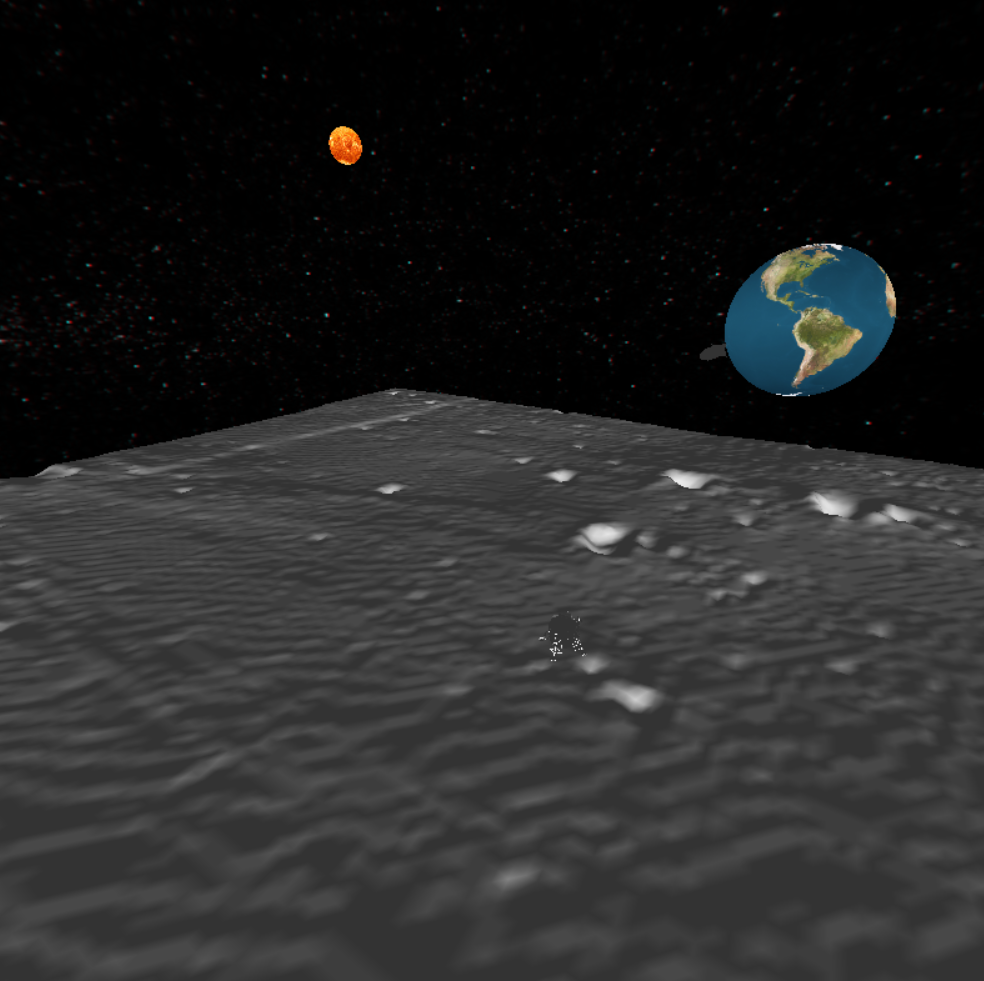
\includegraphics[width=0.5\textwidth]{View1.eps}
    \caption{Apollo 11 Alpha - View 1: Lunar Surface}
    \label{fig:View 1}
\end{wrapfigure}



On Thursday, January 3rd, our design group traveled to OMSI with Mike Bailey to meet with Jim Todd in person for the first time. We were treated to a full tour of the Harry C. Kendall Planetarium at OMSI and got to see the inner workings of their setup. We learned that the planetarium received a software upgrade about a year ago and now used DigitalSky: Dark Matter, a software produced by SkySkan, a provider of planetarium equipment and services. Jim showed us the Dark Matter interface on the main control computer and we got to see many different samples. This gave us a much better idea of how our project would look on a domed theater and how to best design the project to make the best use of the theater. 

At the time of our visit, our group's plan was to animate all portions of the Apollo 11 mission, from launch to splashdown. However, when talking with Jim, we changed course to instead focus more on what happened on the Moon's surface and instead use original news footage to depict what happened before and after. We have some creative freedom with specifics, but our current story board is now as follows: 

\begin{itemize}
    \item The animation will start with original video of the launch, show a flight path of the Saturn V rocket to the Moon, include audio snippets of relevant quotes, and then show the Lunar Lander descending onto the lunar surface.
    
    \item The operator will now be able to interact with the animation, changing the view of the camera on the lunar surface. If no changes are made, the camera will follow a simulation of what Neil Armstrong did on the surface through his eyes. Key points will include: first steps on the surface, planting the American Flag, views of the Earth, and more. During this time, the operator will be able to take questions from the audience. 
    \item When the Operator is ready to end the animation, they will begin a scripted ending where Neil gets back in the Lunar Module and ascends from the surface, show the flight path again, show the Saturn V Rocket, audio snippets of relevant quotes, and then video of the splashdown on Earth, finishing with credits. 
\end{itemize}

Our group will implement this animation in OpenGL. Unfortunately, we recently discovered this will not work directly with the DigitalSky system at OMSI. Instead, we will need to translate our animation into a unique scripting language for use in the planetarium. This will be good because we will be able to make full use of the software's capabilities, but could result in some complications when trying to convert our project to that language. Mike Bailey has been, and is currently in contact with Jim Todd and a contact with SkySkan to find the best ways to complete this conversion. Converting our animation into the scripting language has been added as a stretch goal for our project.\newline\newline


\section{Current Progress}

\begin{wrapfigure}{l}{0.4\textwidth}
    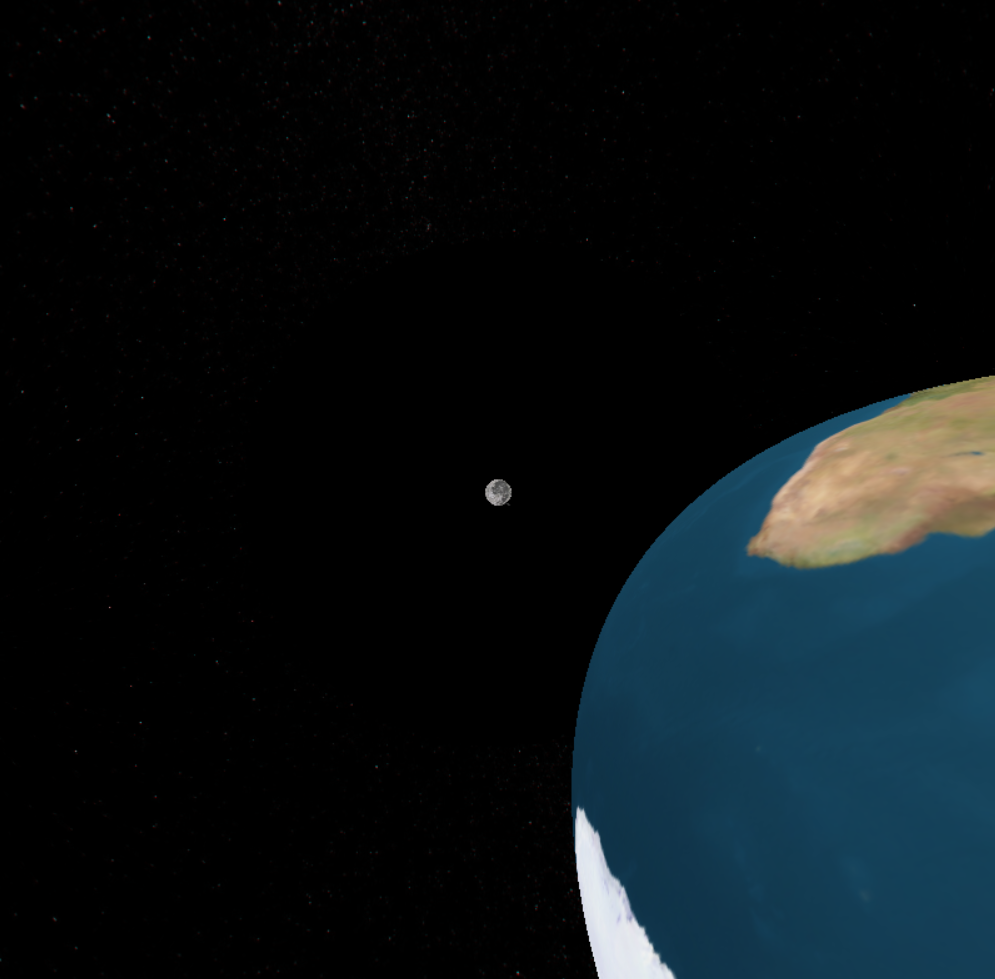
\includegraphics[width=0.4\textwidth]{View2.eps}
    \caption{Apollo 11 Alpha - View 2: From Earth}
    \label{fig:View 2}
\end{wrapfigure}

As of February 24th, our team has created a program in OpenGL that has the main scene of the Apollo 11 mission on the lunar surface. The lunar surface is placed at the origin and has the lunar module and an astronaut placed on it. These objects have been obtained from NASA's 3D object repository online. Textures were included with these files, but we are still working on parsing those files to retrieve the data we need to get the textures working. The Saturn V rocket has also been loaded in, but we are unsure if that will be included in our final release because most of the rocket never left the atmosphere of the Earth. 

The Moon, Earth, and Sun are included in the scene with a star map making up the background. We were able to accurately position and scaled the Moon and Earth, but the numbers for the Sun had to be manipulated. If we had not changed the numbers, the program would have to use many more resources to accurately represent the true position/scale of the Sun. 

Currently, there are six viewpoints highlighting different views either on the lunar surface, or from viewpoints in space, each of which are included in this document. These viewpoints are bound to 1-6 on a keyboard. Also, the 'A' key will play an audio clip from the Apollo 11 mission, showing audio functionality.  

\section{To Do}

\begin{wrapfigure}{r}{0.4\textwidth}
    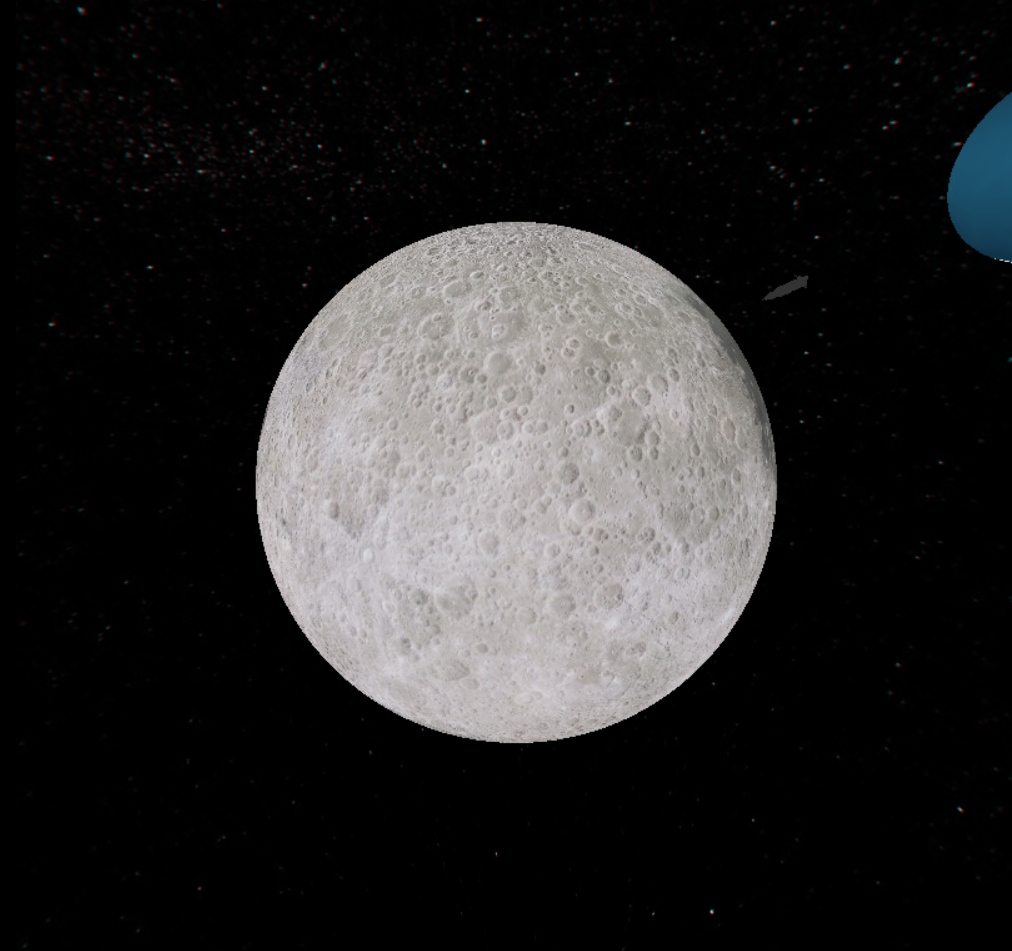
\includegraphics[width=0.4\textwidth]{View3.eps}
    \caption{Apollo 11 Alpha - View 3: Moon}
    \label{fig:View 3}
\end{wrapfigure}

To reach the level of alpha, we created the scene in which our animation would be shown. For beta level functionality, we need to make the scene come to life. To do this one of our first goals is to place all objects as accurately as possible, mainly making sure that the landing site is at the correct location on the Moon and that the Earth is at the correct angle when looking from the Moon. Also, currently the Earth is a single texture, but realistically, there are clouds and shadows on the Earth, which will need to be added. There will also be fine tuning to lighting to make the scene on the lunar surface as close to life-like as possible.

To take this project from a static scene to an animation that can be shown at OMSI, we will focus on adding more viewpoints that are made with key-frame animation so that the viewer is flown throughout the scene. This will be how the operator will mainly show the animation at the expo or OMSI. Then, more audio snippets will be added and our hope it to be able to include historic videos of the Apollo 11 mission. These will give the audience a better idea of what the astronauts and the rest of the world were thinking during this mission. 

\begin{wrapfigure}{r}{0.4\textwidth}
    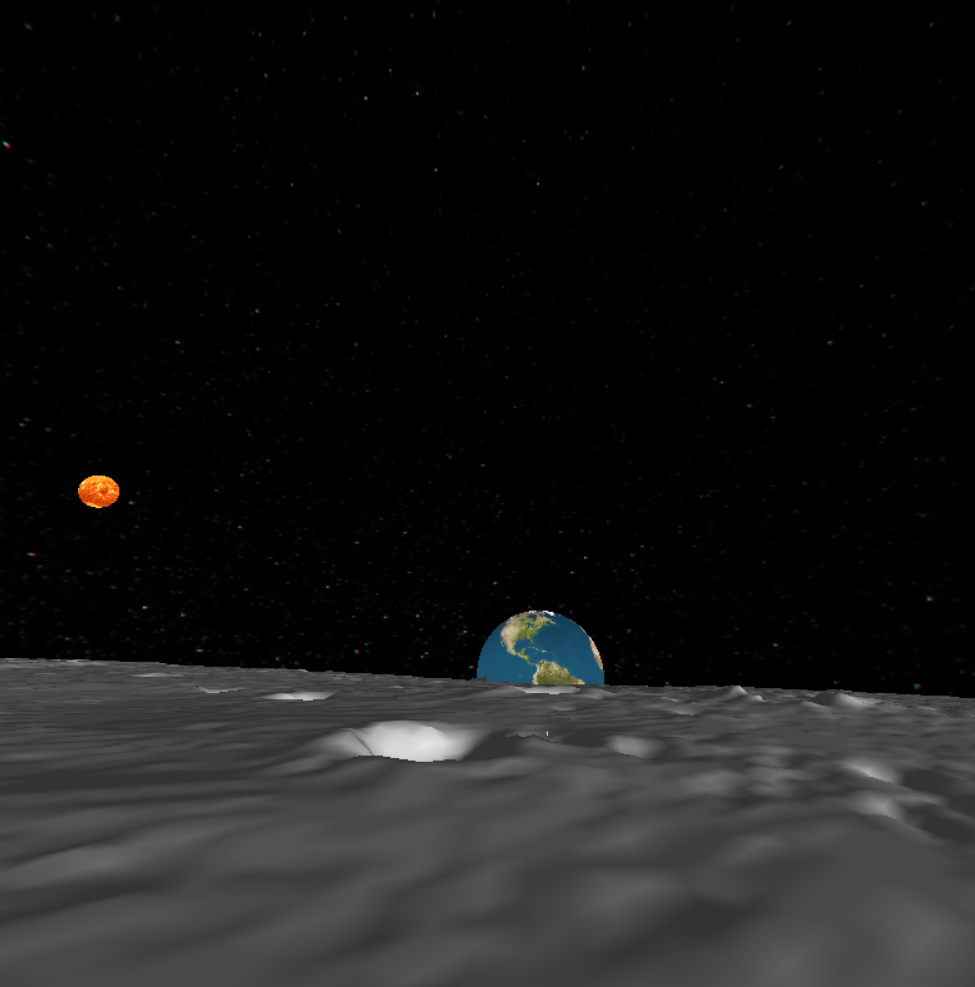
\includegraphics[width=0.4\textwidth]{View4.eps}
    \caption{Apollo 11 Alpha - View 4: From Lunar Module}
    \label{fig:View 4}
\end{wrapfigure}

One object that was not included in the alpha was the iconic American flag on the lunar surface. There were no online resources for a 3D object of that flag, so our group will need to make one ourselves. In addition to this, there are other object that we would like to include on the surface such as the various experiment stations that were used; but these are stretch goals because those would be very complex to model without other resources. Then, an overall goal is to make sure that all objects are textured and look as realistic as possible.

\section{Problems and Solutions}

One of the problems our group has encountered obtaining quality 3D objects for our scene. Luckily, NASA has a Github that contains .stl files for 3D objects from most of their missions. We obtained the models for the Saturn V, lunar module, astronaut, and lunar surface. However, these models were not to scale, so our group is continuing to adjust their sizes so they are more accurate. Another problem our group has encountered was implementing audio. The API we were planning on using uses a heavily deprecated library and the functions to play audio were not working. Instead, our group is currently using a Windows function to play audio files, making it so only computers with Windows OS can play audio. We are unsure how we will integrate audio into the planetarium at OMSI, but we believe that there will be built in functionality there. 

\begin{wrapfigure}{l}{0.4\textwidth}
    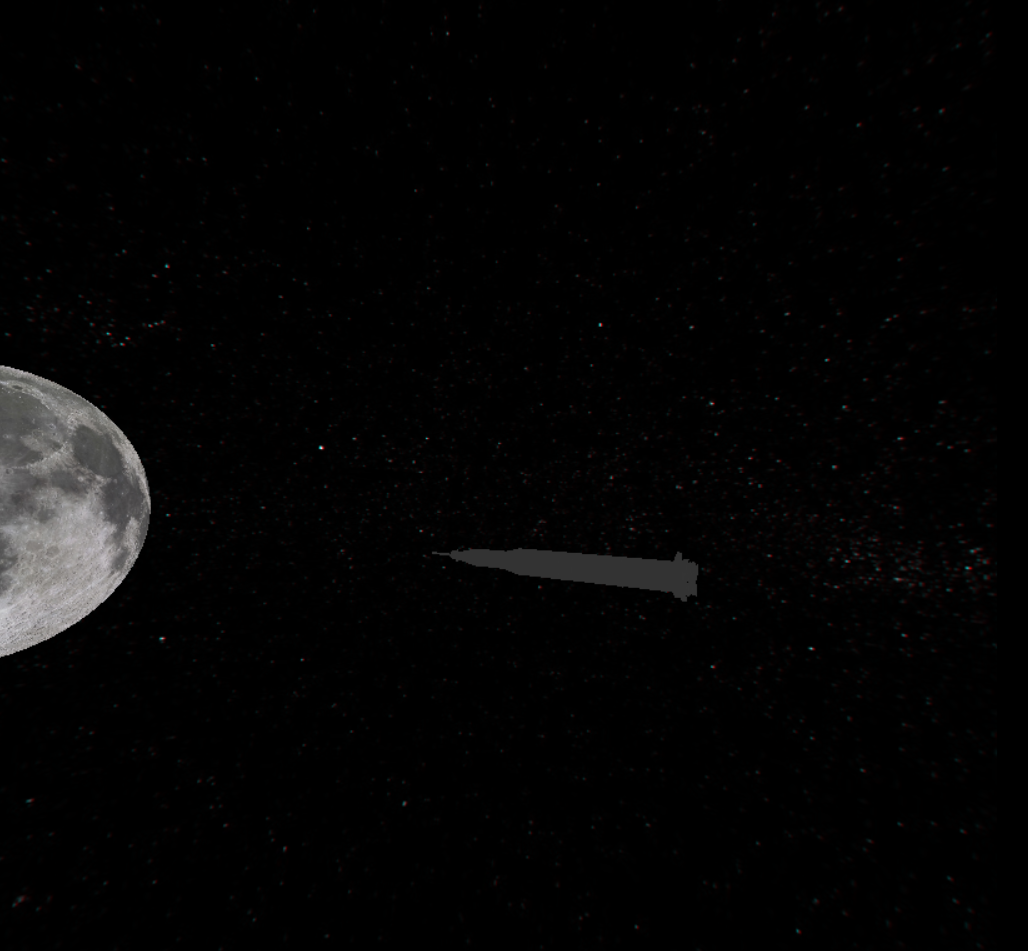
\includegraphics[width=0.4\textwidth]{View5.eps}
    \caption{Apollo 11 Alpha - View 5: Saturn V}
    \label{fig:View 5}
\end{wrapfigure}

Implementing historical videos was also a problem for our group. We met with Mike Bailey to discuss how we might achieve this. He told us how every frame of a video can be saved in memory and placed onto a quadrilateral object as an image. These images would upload so many frames per second in order to play the entire video. This technique does not play the audio of the video, however, so our group will have to sync the audio file with the video that is playing. Lastly, a more general issue our group encountered was that SkySkan, the company that created the planetarium software, informed us that OpenGL is not directly compatible with their software. Our group decided that creating an OpenGL animation will still be a requirement so that we can show something at the engineering expo. While making the video compatible with the planetarium is still our main focus, for the purposes of priorities, we have moved that to become a stretch goal. That stretch goal is to convert our OpenGL program to a unique scripting language used by the planetarium's software. This should be just like learning a new coding language, but there may be different functionalities that our team will need to navigate. 


\section{Conclusion}

\begin{wrapfigure}{l}{0.45\textwidth}
    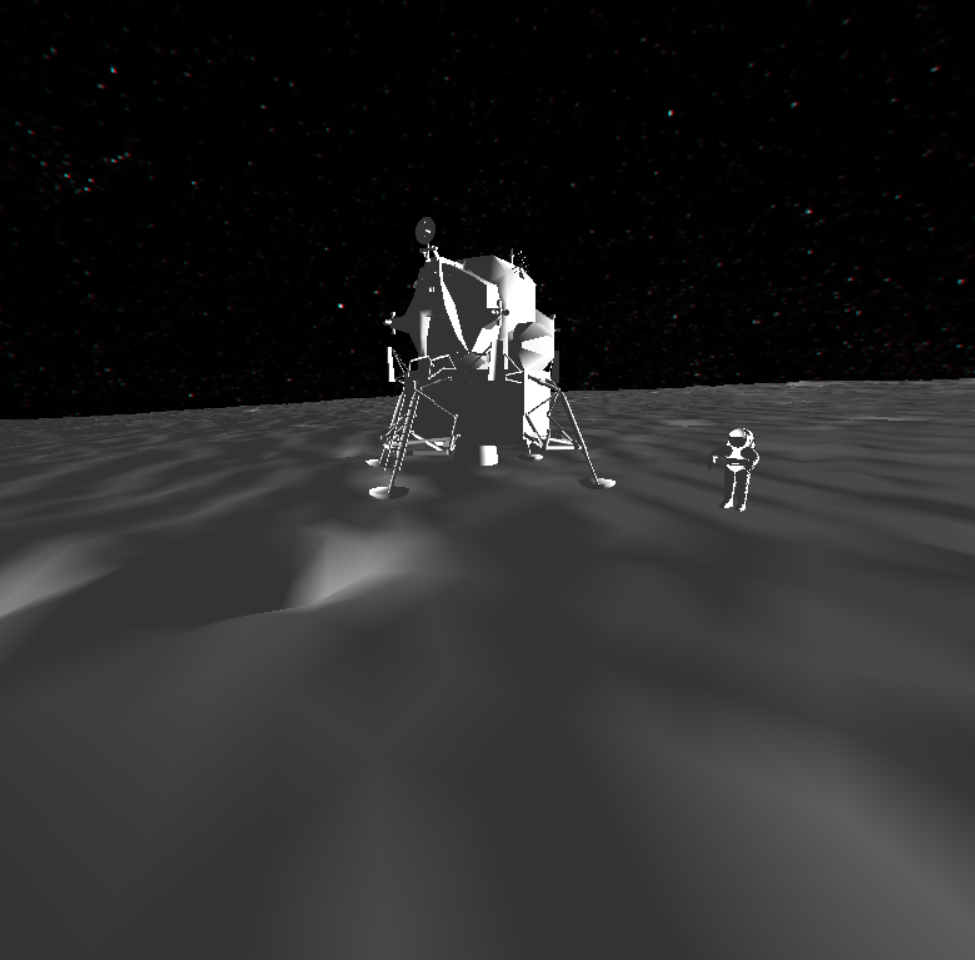
\includegraphics[width=0.4\textwidth]{View6.eps}
    \caption{Apollo 11 Alpha - View 6: Module and Astronaut}
    \label{fig:View 6}
\end{wrapfigure}

\end{document}
